\documentclass{ctexbeamer}
\usetheme{metropolis}
\usepackage{mathpazo}
\usepackage{fontspec}
\setCJKsansfont{方正清刻本悦宋简体.ttf}
\setsansfont{Palatino}
\setmonofont{Consolas}
\usepackage{graphicx}
\usepackage{xcolor}
\definecolor{comment}{RGB}{0,166,82}
\definecolor{keyword}{RGB}{0,174,247}
\definecolor{tip}{RGB}{244,105,102}
\usepackage{amsmath}
\usepackage{amssymb}
\usepackage{physics}
\usepackage{booktabs}
\usepackage{bm}
\usepackage{listings} % 代码美化包
\lstset{
	language=[latex]TeX, breaklines, basicstyle=\ttfamily,
	keywordstyle = \bfseries\color{keyword},
	commentstyle = \color{comment},
	texcsstyle=*\color{keyword}\bfseries
}
\usepackage{multicol}
\usepackage{fontawesome5}
\newcommand\link[1]{\href{#1}{\faLink}}
\newcommand\pkg[1]{\it\texttt{#1}}
\newcommand\CASE[1]{{\addfontfeatures{Letters=Uppercase}#1}}
\setbeamertemplate{bibliography item}[text]

\begin{document}
% xelatex --synctex=1 Lecture.tex
\title{\LaTeX 从入门到入门}
\date{\today}
\author{彭康学导团志愿者部 \quad 核工A002班 \quad 张恺 \faRadiation*}
\institute{彭康书院学业辅导与发展中心}
\titlegraphic{\hfill
\includegraphics[height=2cm]{figures/logo.png}}
\maketitle

\begin{frame}[standout]
  \huge 提前声明 \\[1ex]
  \footnotesize 本次讲座主要针对彭康学导团真题整理工作,无法介绍\LaTeX{}全貌
\end{frame}

\section{简单介绍}

\begin{frame}{什么是\LaTeX ?}
  \begin{itemize}
    \item \TeX 是由Donald E. Knuth为排版文字和数学公式而开发的软件。
    \item \LaTeX 是一种使用\TeX 程序作为排版引擎的格式,可以粗略地理解为\LaTeX 是\TeX 的一层封装,由Leslie Lamport开发。
  \end{itemize}
  \begin{columns}
    \begin{column}{0.45\textwidth}
      \begin{figure}
        \centering
        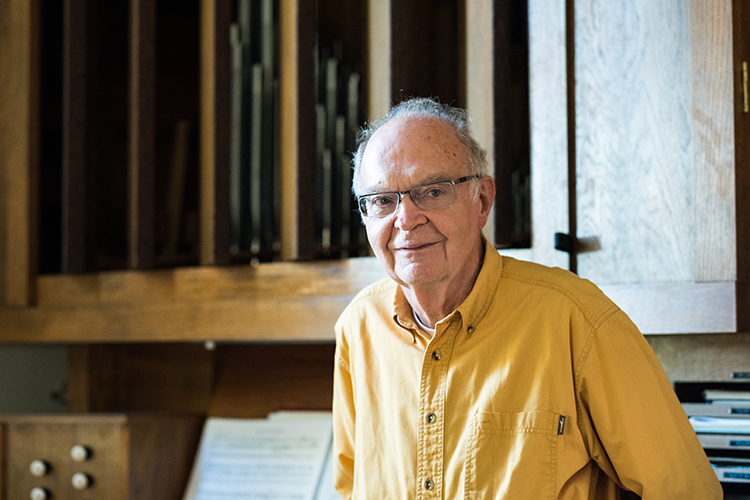
\includegraphics[height=2.8cm]{figures/Knuth-vivian20181019E.jpg}
        \caption{Donald E. Knuth(\TeX)}
      \end{figure}
    \end{column}
    \begin{column}{0.45\textwidth}
      \begin{figure}
        \centering
        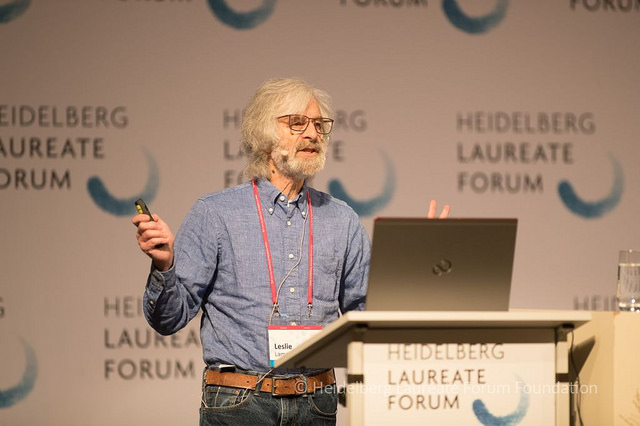
\includegraphics[height=2.8cm]{figures/lamport-2018.jpg}
        \caption{Leslie Lamport(\LaTeX)}
      \end{figure}
    \end{column}
  \end{columns}
  \nonumberfootnote{\scriptsize 图片来源:
    \link{https://www-cs-faculty.stanford.edu/~knuth/graphics.html}
    \link{https://aperiodical.com/2018/09/hlf-blogs-leslie-lamport-thinks-your-code-is-bad}}
\end{frame}

\begin{frame}{\LaTeX~or~Word ?}
  \begin{itemize}
    \item \LaTeX
          \begin{itemize}
            \item 所想即所得(学习门槛高,想要看到效果需要频繁编译)
            \item 内容和格式分离(格式的调整不太方便)
            \item 强大的数学公式排版(不容易排查错误)
            \item 开源、免费(维护问题)
          \end{itemize}
    \item Word
          \begin{itemize}
            \item 所见即所得(下限低,繁多的标记语言)
            \item 内容和格式混合(难以全身心投入内容创作)
            \item 数学公式兼容性一般(容易造成卡顿)
            \item 收费
          \end{itemize}
  \end{itemize}
  \textcolor{tip}{想法比工具更重要!}
\end{frame}

\begin{frame}[fragile]
  \frametitle{举个简单的例子}
  \begin{columns}
    \begin{column}{0.48\textwidth}
      \scriptsize
      \begin{lstlisting}
\documentclass{ctexart}
\usepackage{amsmath,amssymb}
\begin{document}
\title{彭康学导团\LaTeX 讲座测试}
\author{彭康学导团志愿者部}
\date{\zhtoday}
\maketitle
\section{测试第一节}
你好,\LaTeX !
\[
f(q)=-\frac{m}{2\pi\hbar^2}\int V(r){\rm e}^{iqr/\hbar}{\rm d}r
\]
\section{测试第二节}
\begin{enumerate}
  \item 这是第一点
  \item 这是第二点
\end{enumerate}
\end{document}
  \end{lstlisting}
    \end{column}
    \begin{column}{0.48\textwidth}
      \begin{figure}
        \centering
        \vspace{-0.8cm}
        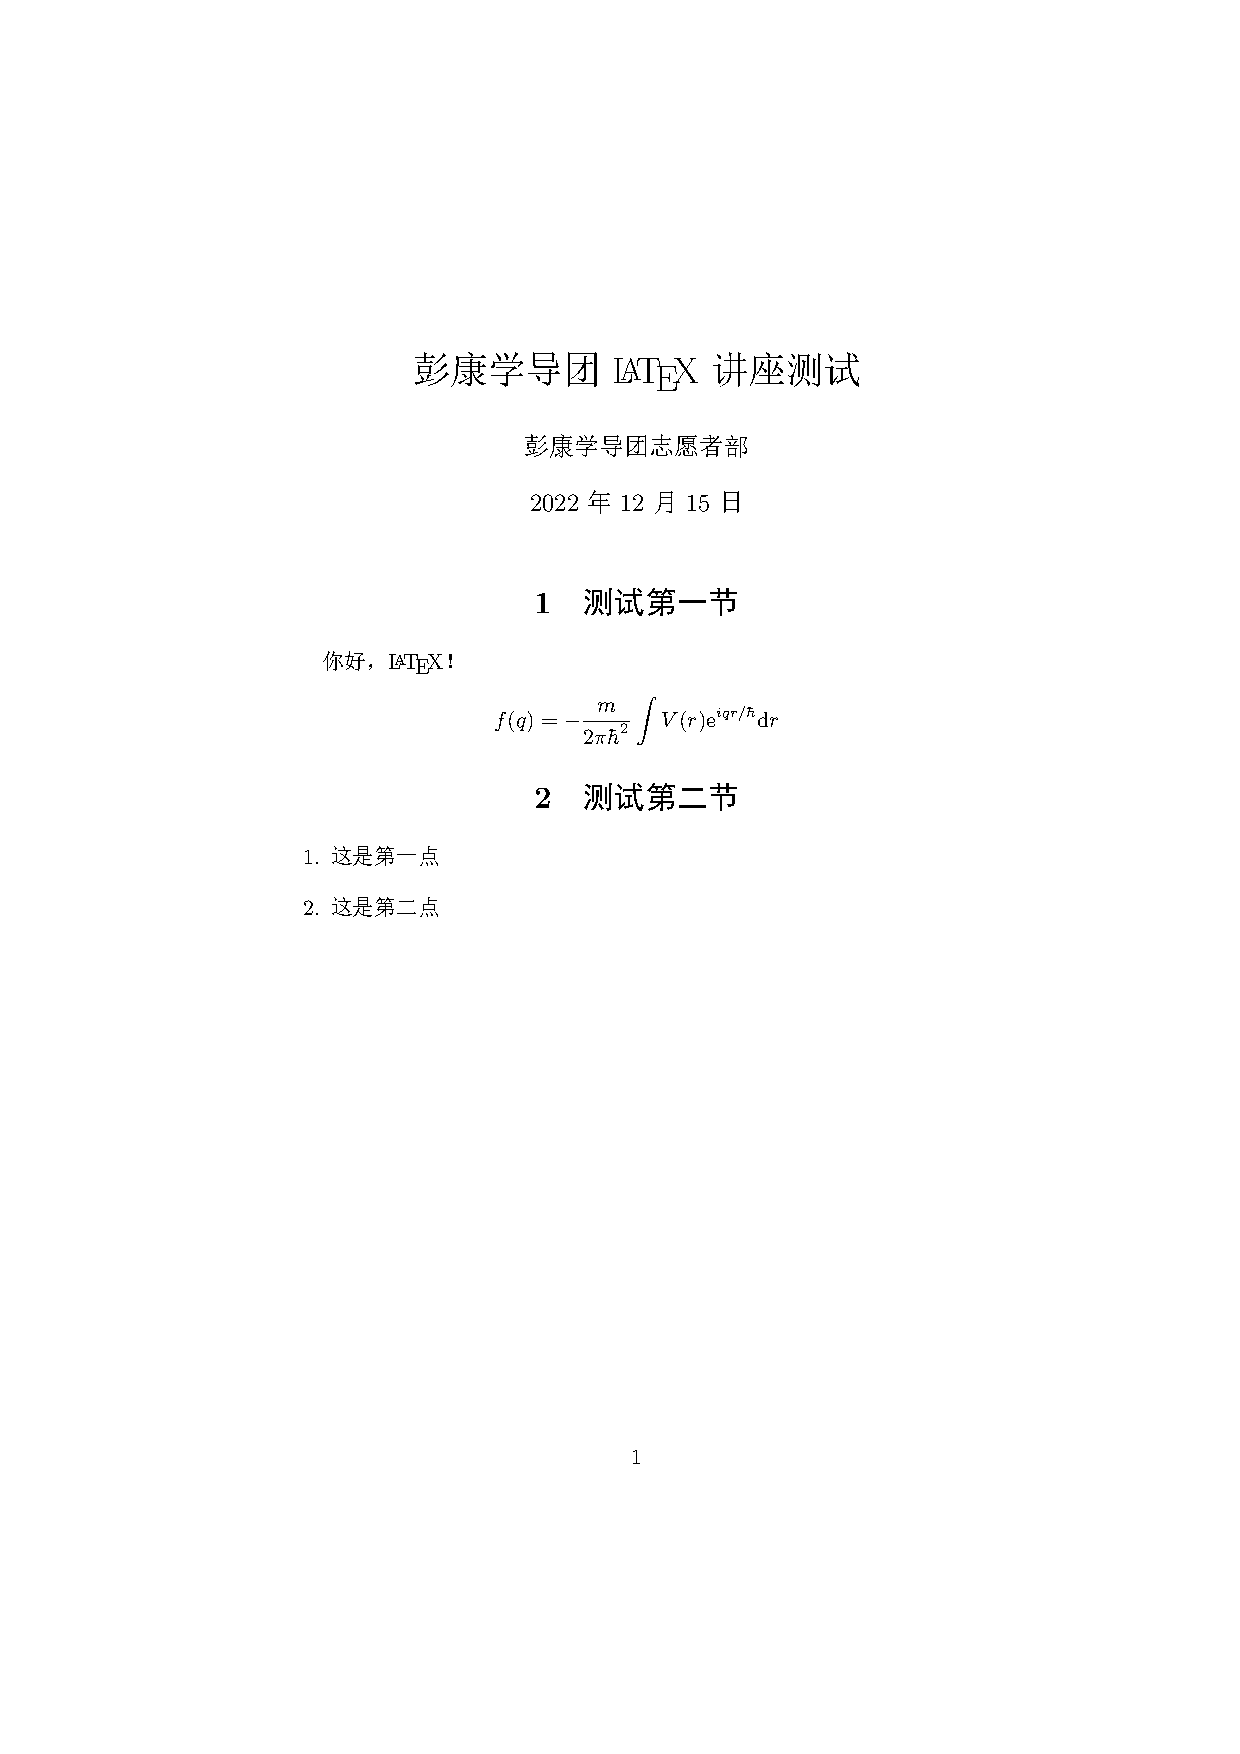
\includegraphics[width=\textwidth]{figures/test1.pdf}
      \end{figure}
    \end{column}
  \end{columns}
\end{frame}
\section{PKSTU}
\begin{frame}{彭康学导团现有的以\LaTeX 排版的资料}
    \begin{itemize}
        \item 大学物理(上)笔记 \link{https://github.com/PKSTU/University-Physics-Notes.git}
        \begin{columns}
            \begin{column}{0.48\textwidth}
                \begin{figure}
                    \centering
                    
\includegraphics[scale=0.2]{figures/PK_DW1.pdf}
                \end{figure}
            \end{column}
            \begin{column}{0.48\textwidth}
                \begin{figure}
                    \centering
                    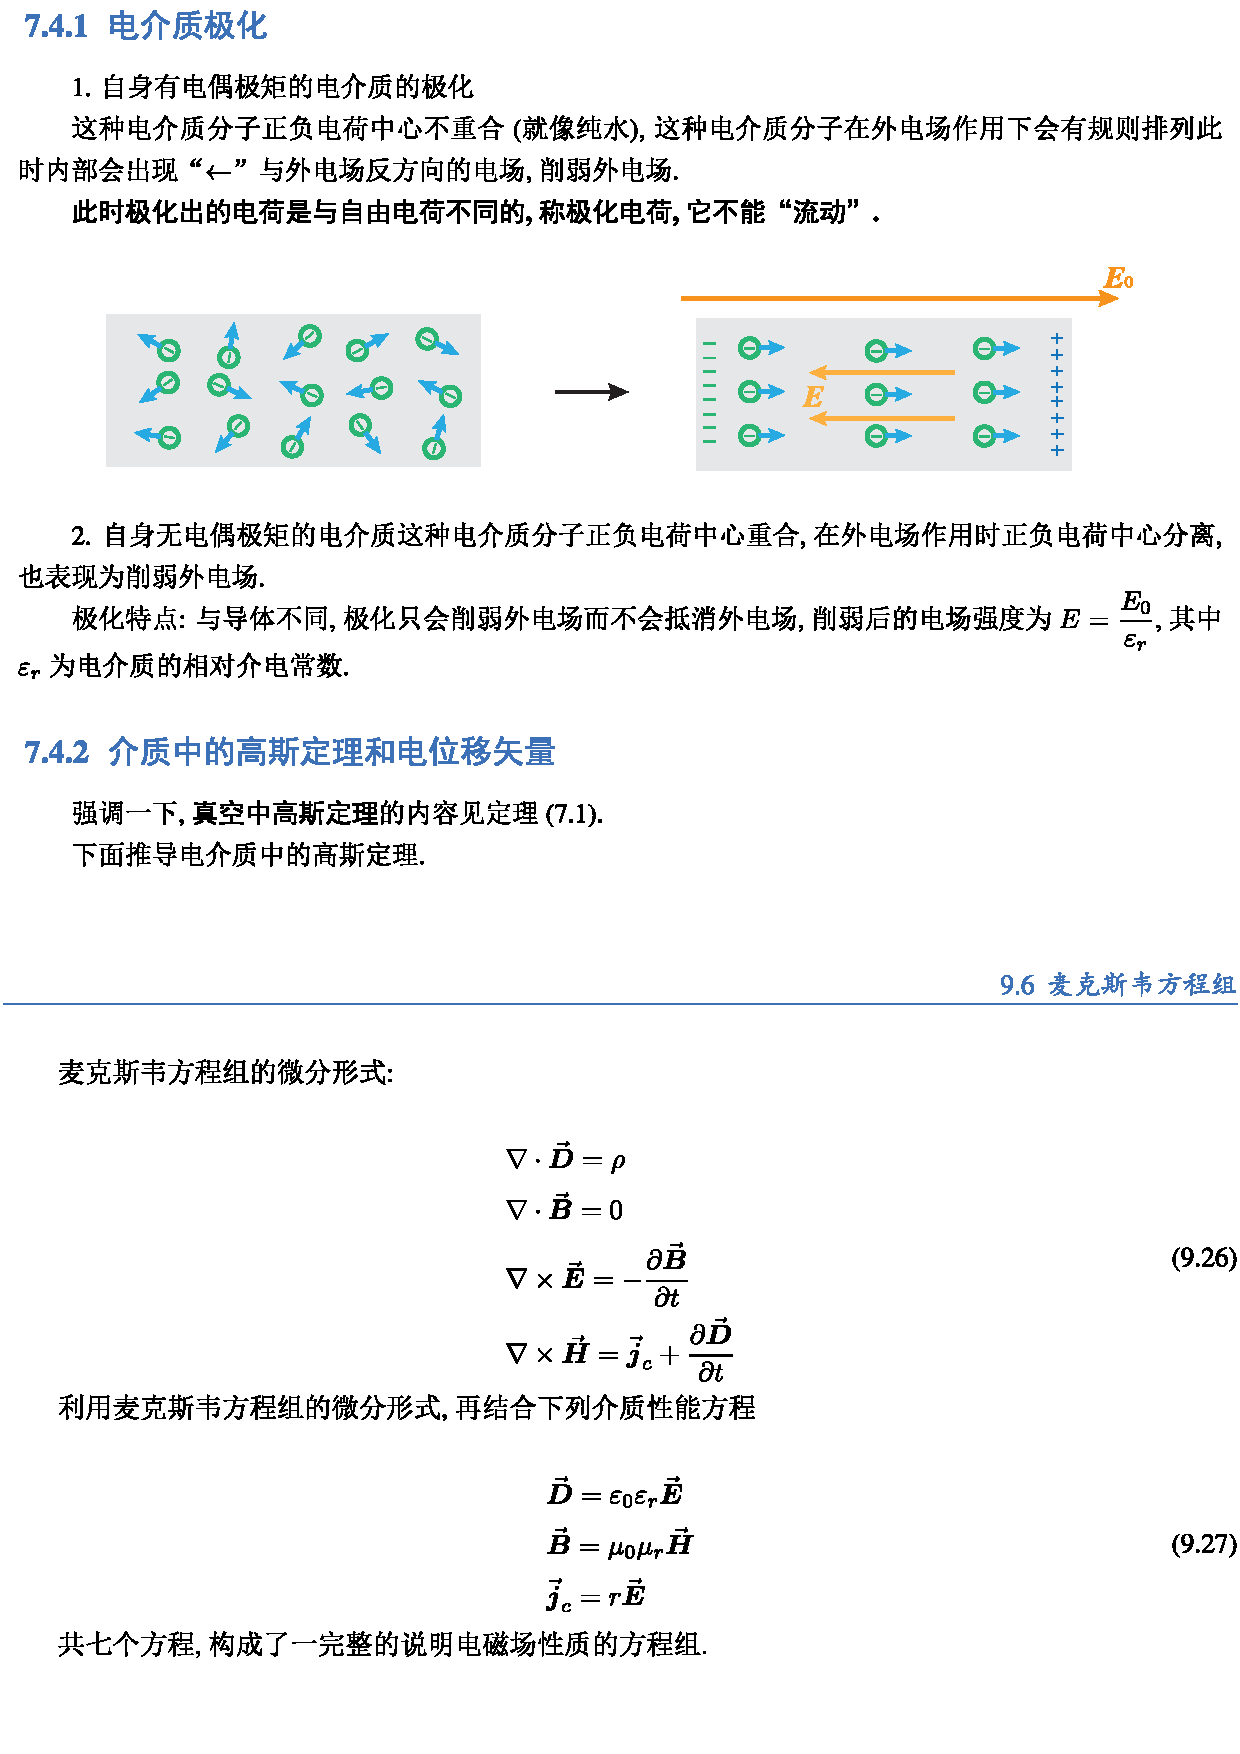
\includegraphics[scale=0.2]{figures/PK_DW2.pdf}
                \end{figure}
            \end{column}
        \end{columns}
    \end{itemize}
\end{frame}

\begin{frame}{彭康学导团现有的以\LaTeX 排版的资料}
    \begin{itemize}
        \item 高等数学(上)\& 线性代数入门讲义 \link{https://github.com/PKSTU/Advanced-Mathematics-Notes.git} \link{https://github.com/PKSTU/Linear-Algebra-Notes.git}
        \begin{columns}
            \begin{column}{0.48\textwidth}
                \begin{figure}
                    \centering
                    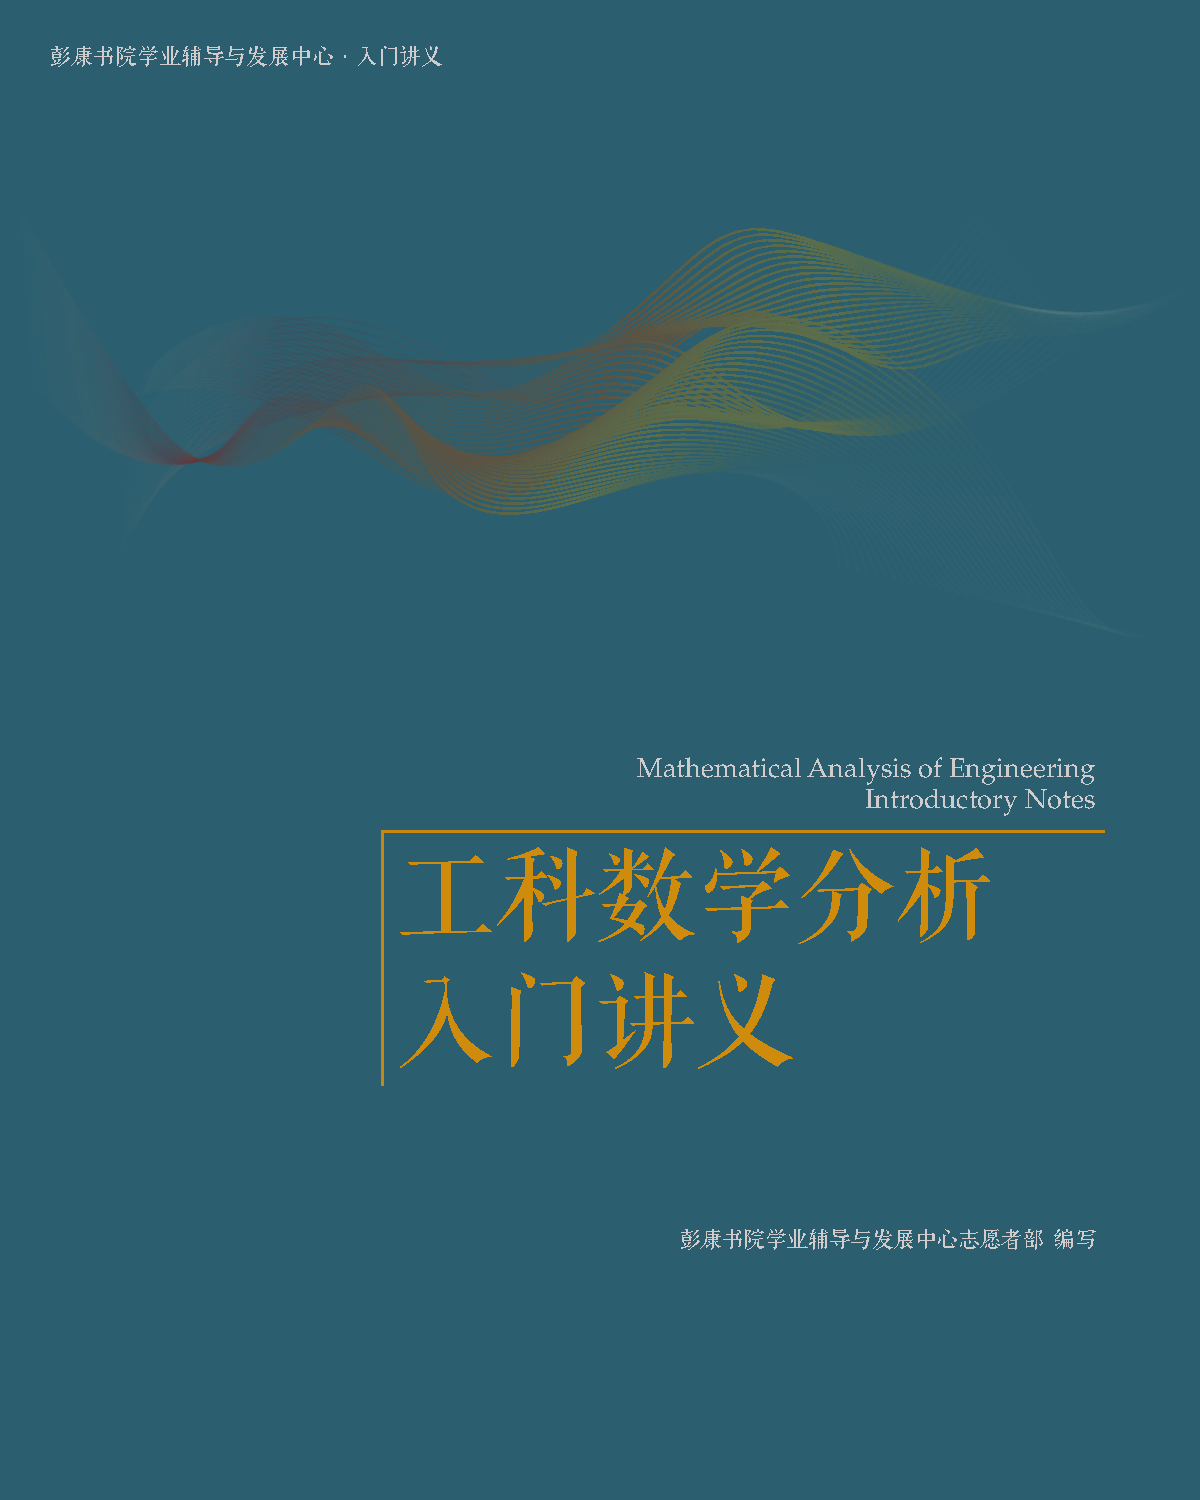
\includegraphics[scale=0.2]{figures/PK_GS.pdf}
                \end{figure}
            \end{column}
            \begin{column}{0.48\textwidth}
                \begin{figure}
                    \centering
                    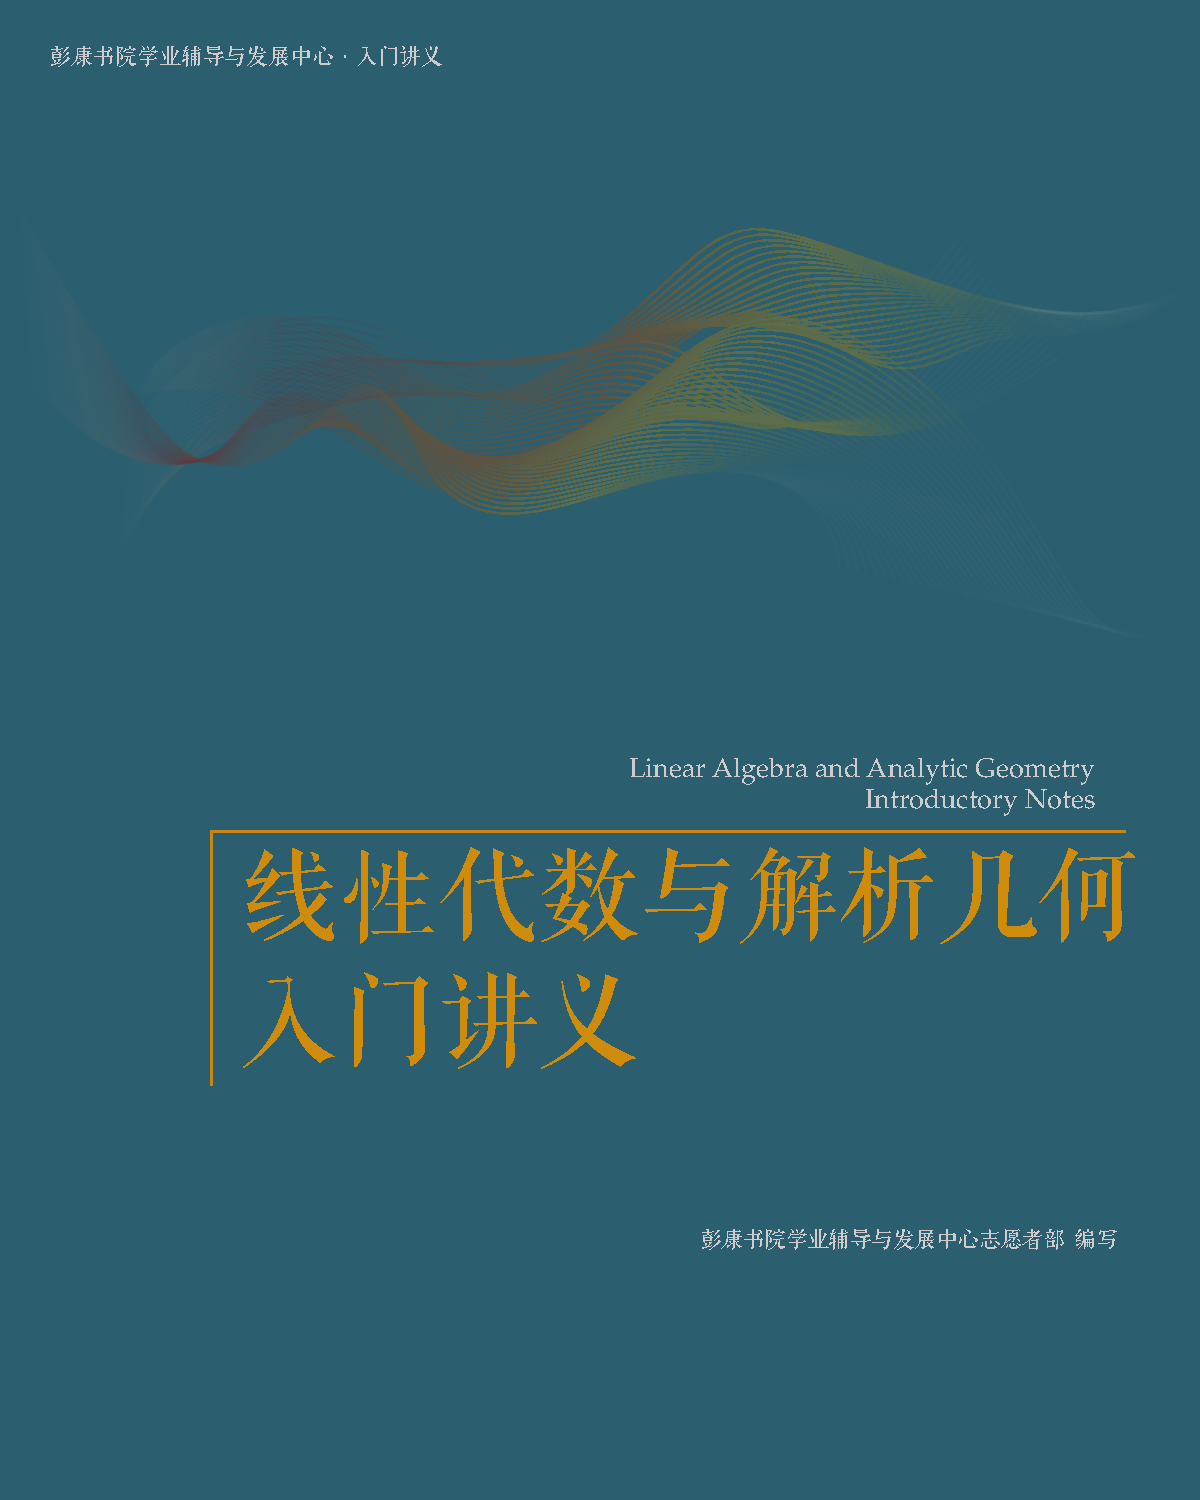
\includegraphics[scale=0.2]{figures/PK_XD.pdf}
                \end{figure}
            \end{column}
        \end{columns}
    \end{itemize}
\end{frame}

\begin{frame}{彭康学导团现有的以\LaTeX 排版的资料}
    \begin{itemize}
        \item 流体力学复习要点 \link{https://github.com/PKSTU/Hydrodynamics-Key-Points.git}
        \begin{columns}
            \begin{column}{0.48\textwidth}
                \begin{figure}
                    \centering
                    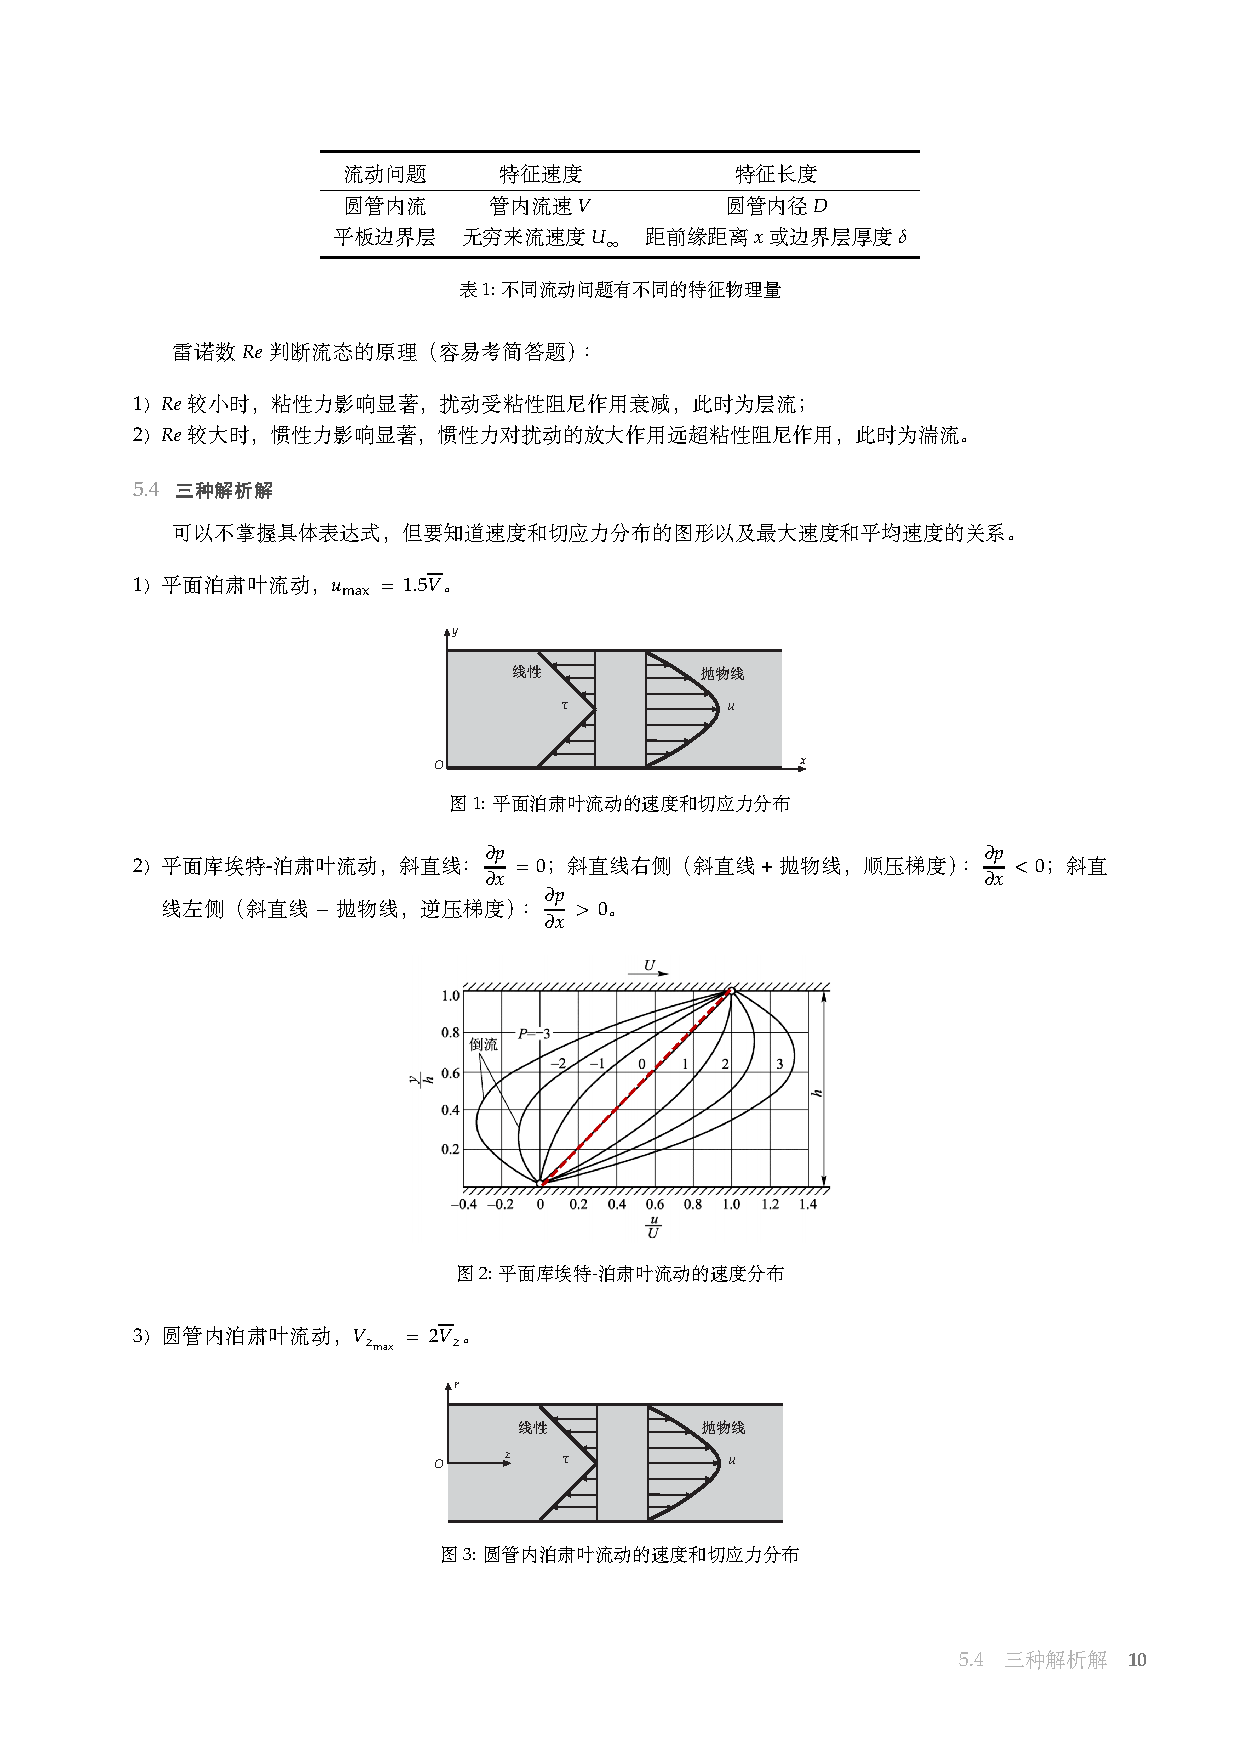
\includegraphics[scale=0.2]{figures/PK_LL1.pdf}
                \end{figure}
            \end{column}
            \begin{column}{0.48\textwidth}
                \begin{figure}
                    \centering
                    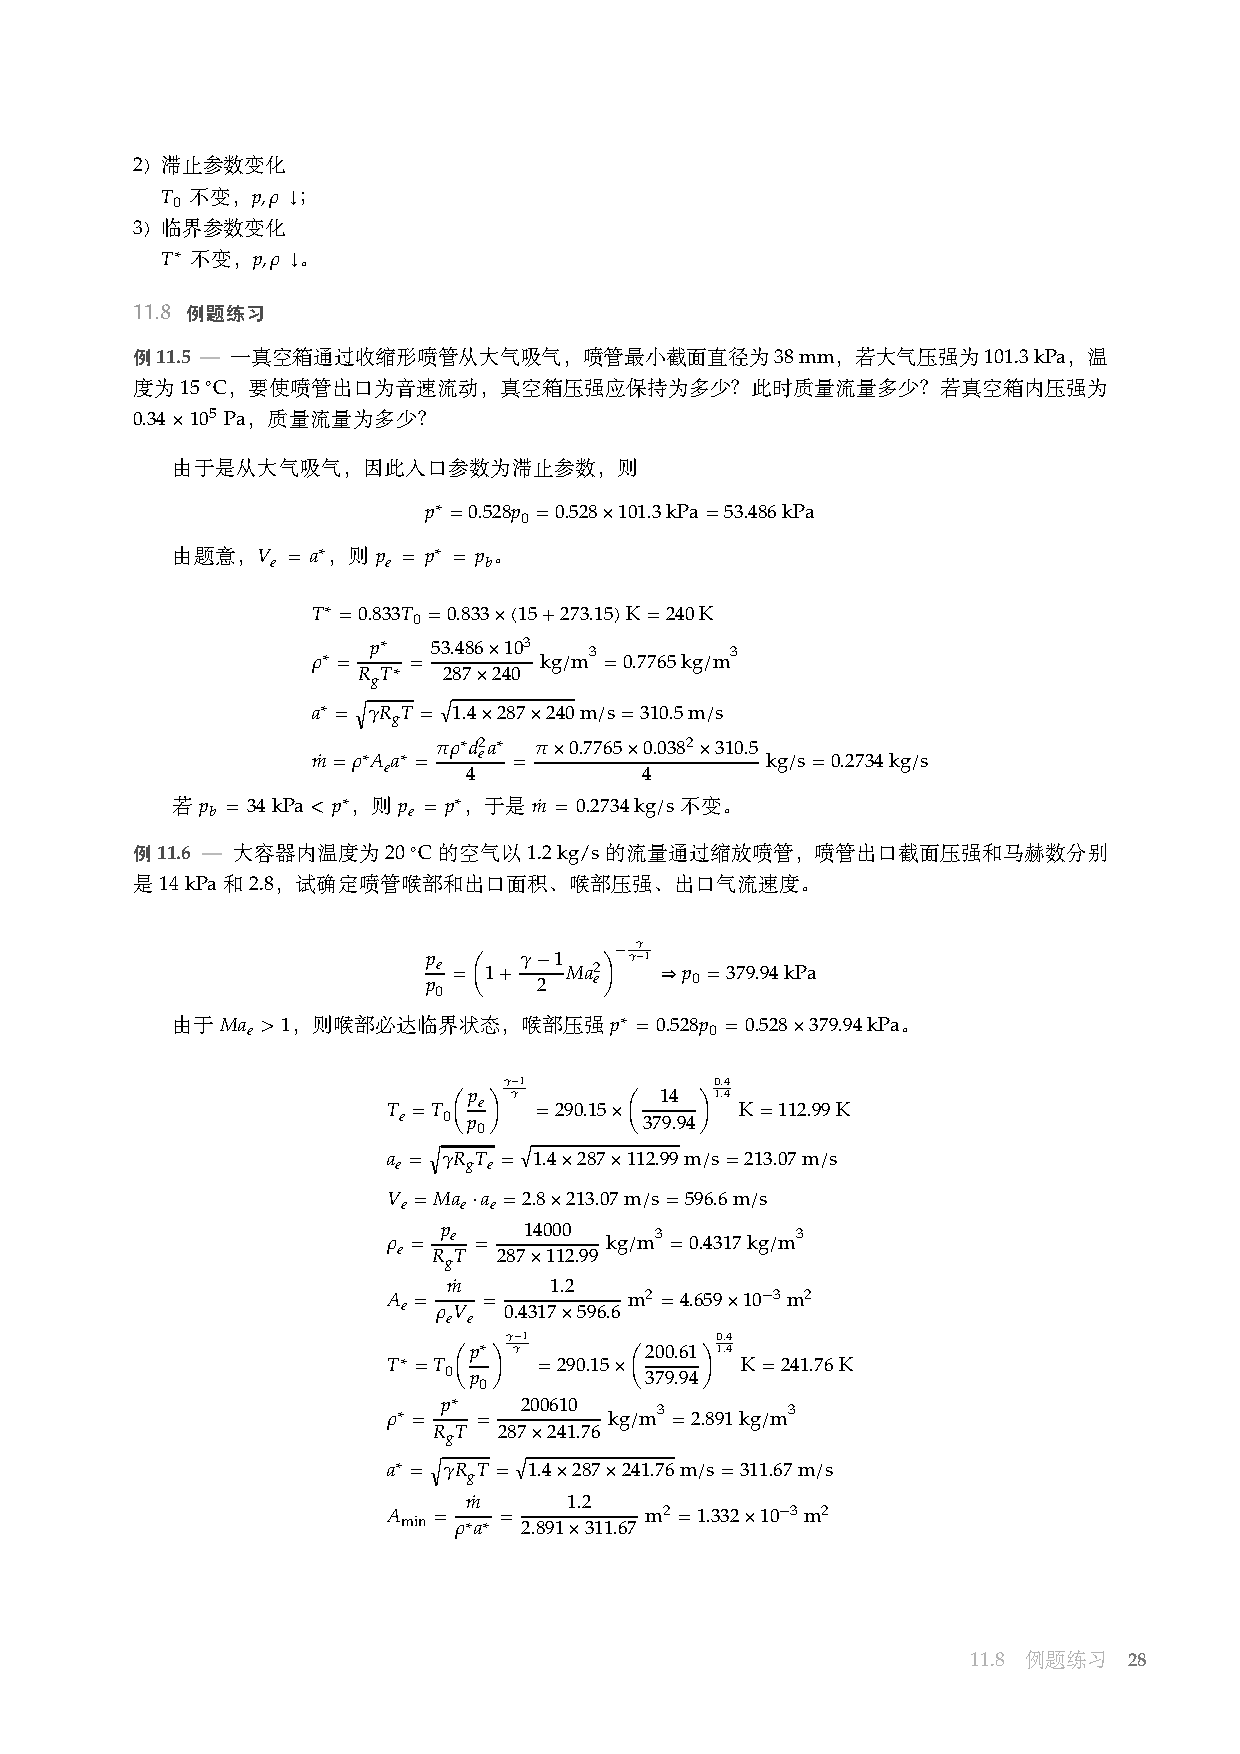
\includegraphics[scale=0.2]{figures/PK_LL2.pdf}
                \end{figure}
            \end{column}
        \end{columns}
    \end{itemize}
\end{frame}

\begin{frame}{彭康学导团现有的以\LaTeX 排版的资料}
    \begin{itemize}
        \item 最新的高数、线代真题及解析 \link{https://github.com/PKSTU/PKSTU-Exam-Advanced-Mathematics-Linear-Algebra.git}
        \begin{columns}
            \begin{column}{0.48\textwidth}
                \begin{figure}
                    \centering
                    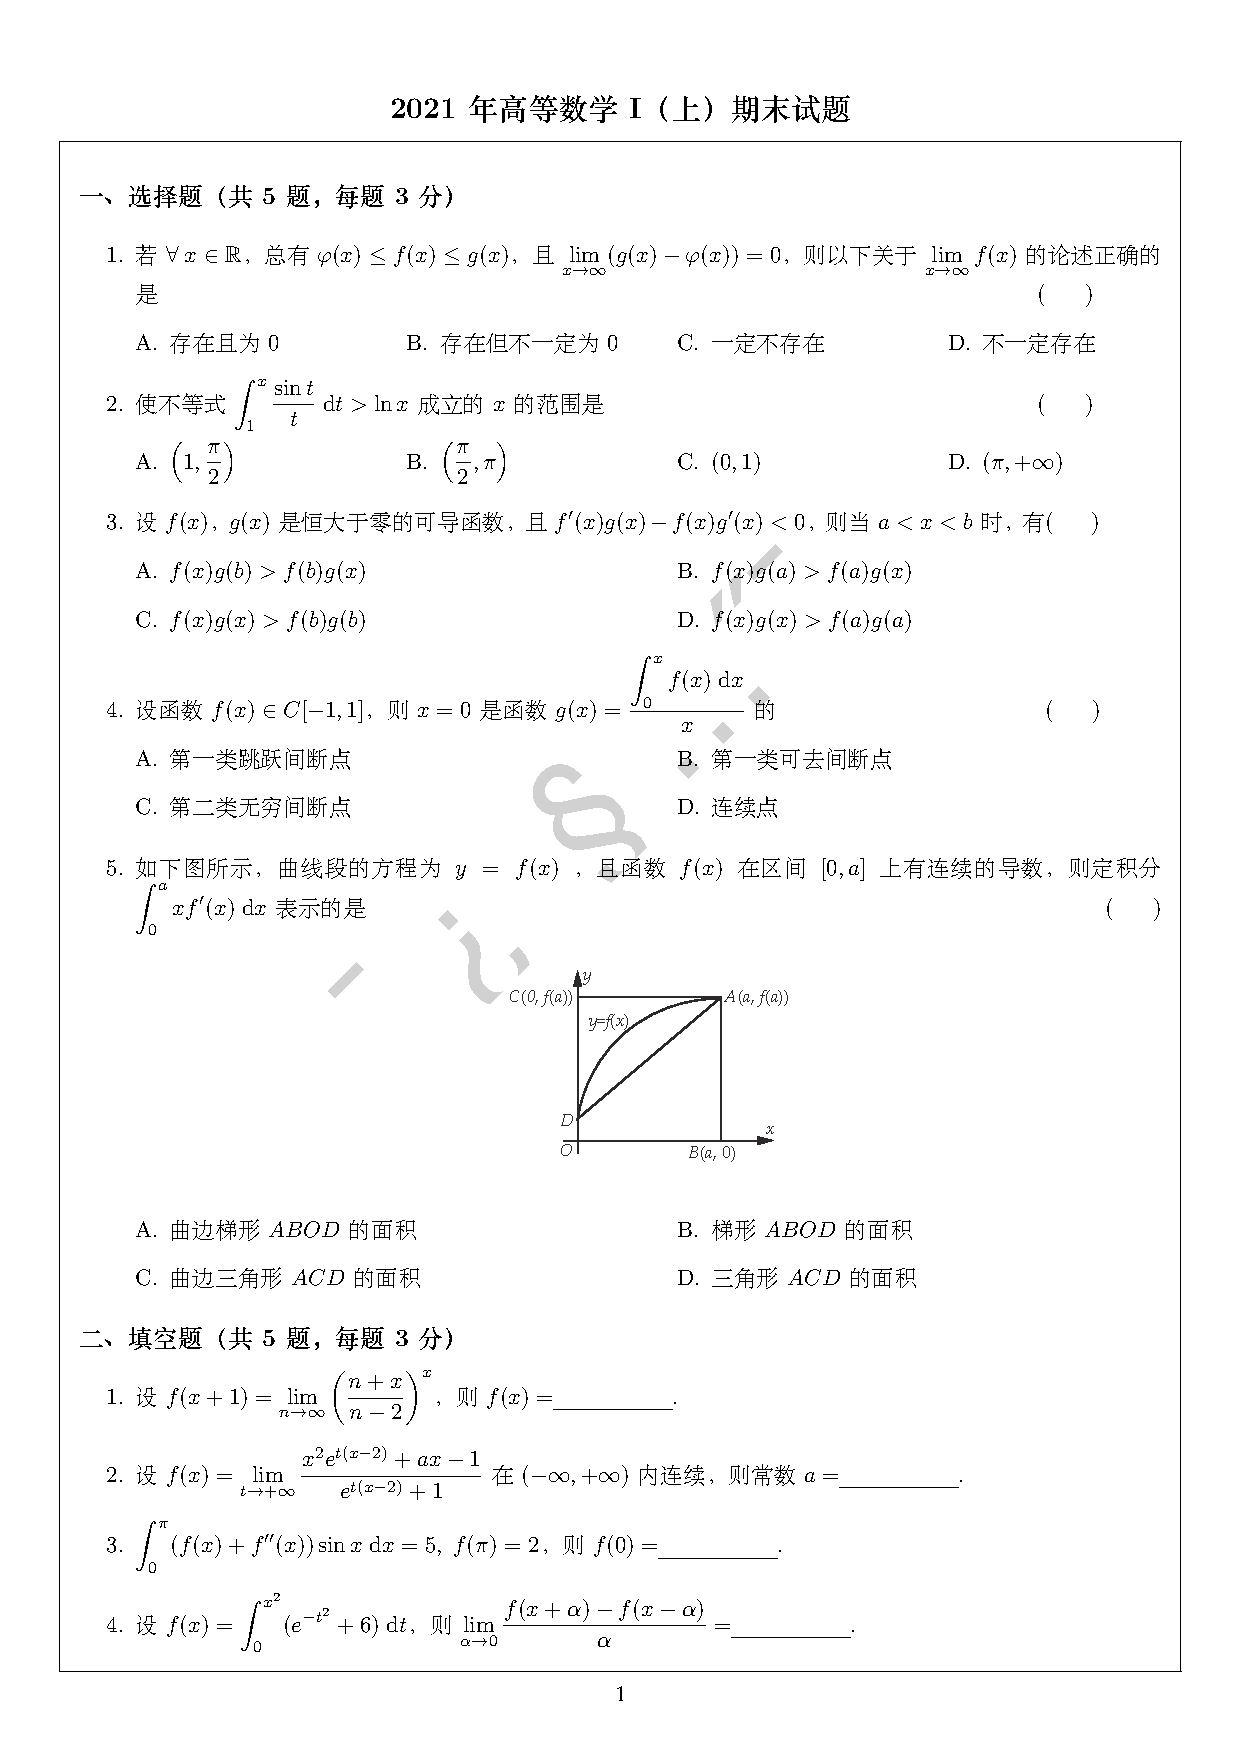
\includegraphics[scale=0.2]{figures/PK_GSZT.pdf}
                \end{figure}
            \end{column}
            \begin{column}{0.48\textwidth}
                \begin{figure}
                    \centering
                    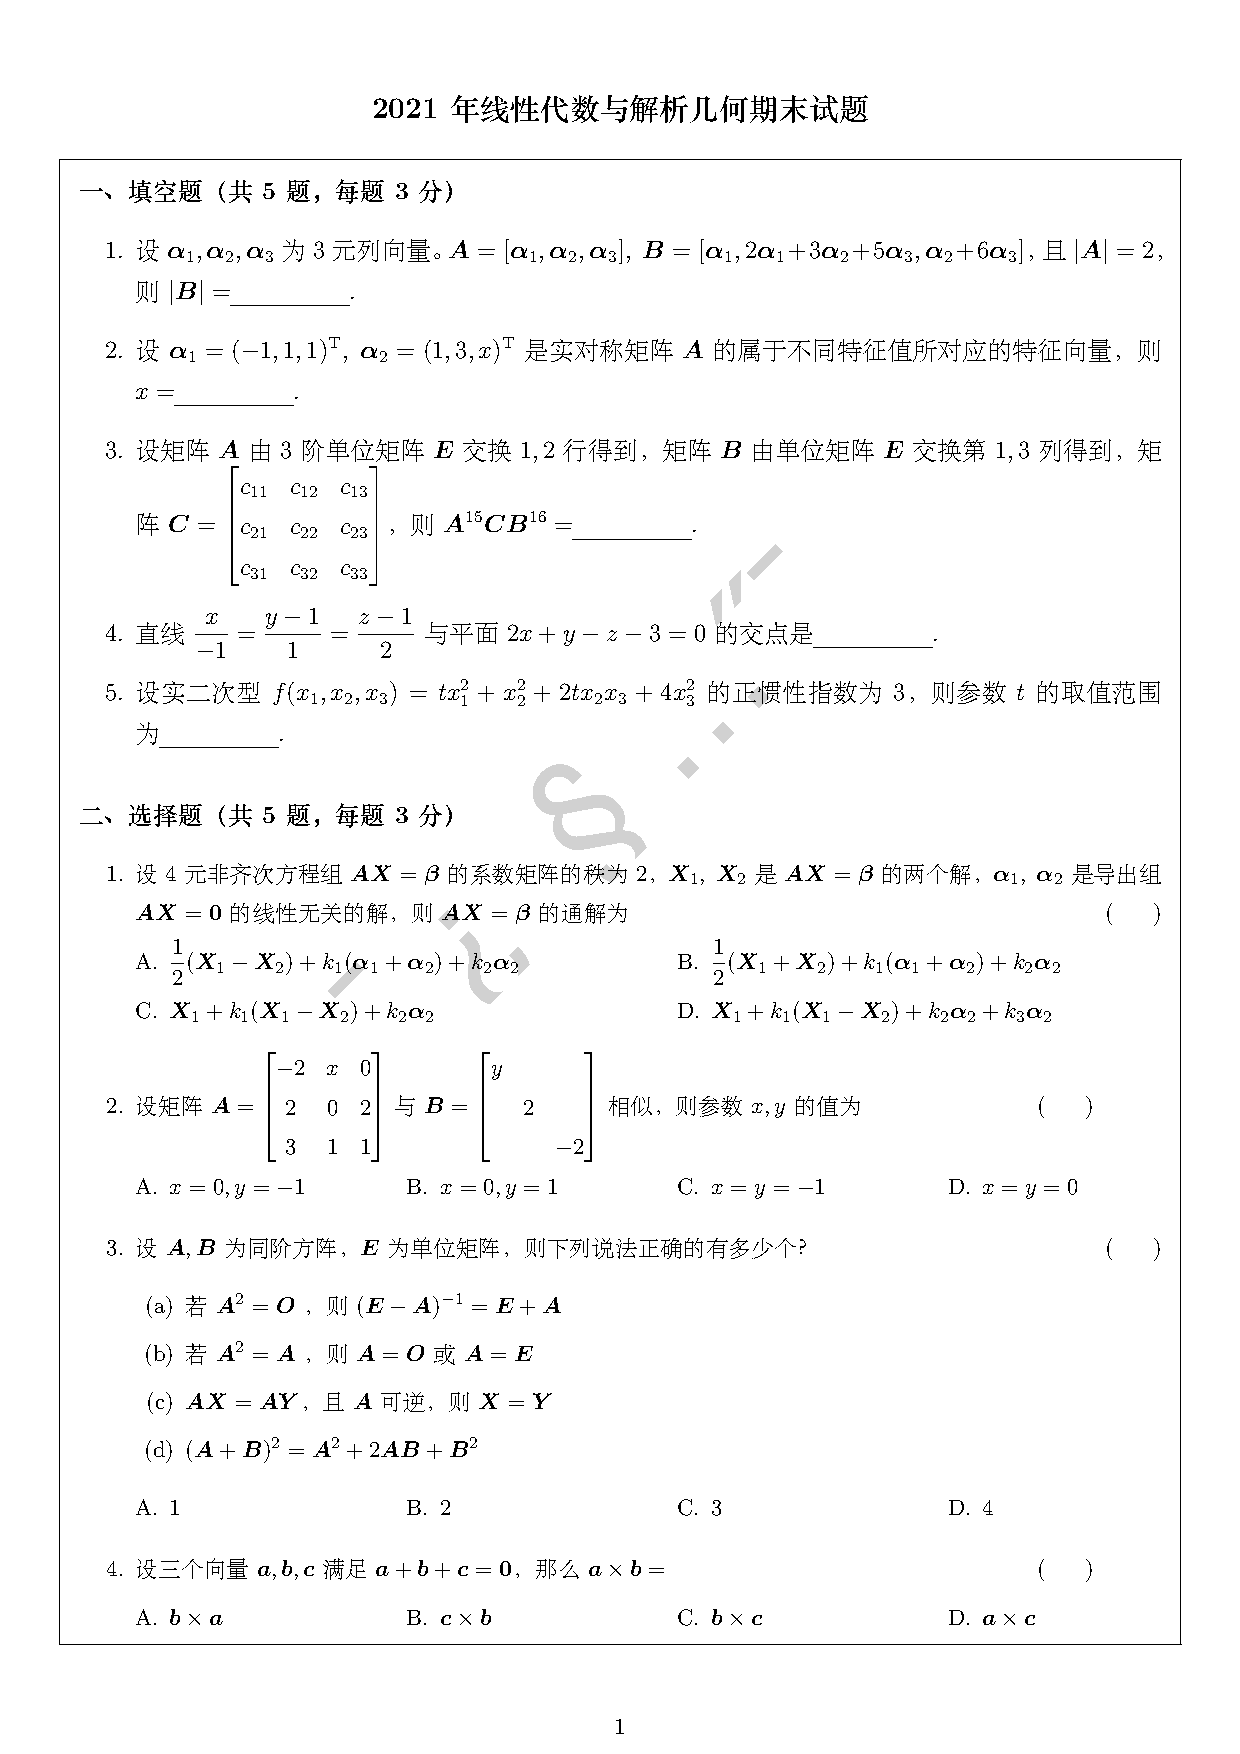
\includegraphics[scale=0.2]{figures/PK_XDZT.pdf}
                \end{figure}
            \end{column}
        \end{columns}
    \end{itemize}
\end{frame}
\section{安装和使用}
\begin{frame}{懒得折腾?}
    \begin{itemize}
        \item 云端服务可能更好用
        \item 免去安装、升级等一系列烦恼,可以多人协作
        \item 版本管理、模板市场等功能要氪金
    \end{itemize}
    \pause
    \begin{columns}
        \begin{column}{0.48\textwidth}
            \begin{itemize}\small
                \item 首推
                      \href{https://www.overleaf.com}{\textcolor[HTML]{138a07}{Overleaf} \faLink}
                      \begin{itemize}
                          \item 模板丰富
                          \item 用户支持很好
                          \item 可能遇到网络问题
                      \end{itemize}
            \end{itemize}
        \end{column}
        \pause
        \begin{column}{0.48\textwidth}
            \begin{itemize}\small
                \item 备选 \\ 
                TeXPage \link{https://www.texpage.com} or Slager \link{https://www.slager.cn/}
                      \begin{itemize}
                          \item 网络限制较少
                          \item 支持更多的中文字体
                          \item 不够成熟稳定
                          \item 免费账号项目数量受限
                      \end{itemize}
            \end{itemize}
        \end{column}
    \end{columns}
\end{frame}

\begin{frame}{选择发行版}
    \begin{itemize}
        \item<+-> \TeX{} 发行版
              \begin{itemize}
                  \item 引擎、宏包、字体、文档的综合体
                  \item \TeX{} Live、Mac\TeX{}、MiK\TeX{} 等
              \end{itemize}
        \item<+-> \TeX{} Live \link{https://www.tug.org/texlive}
              \begin{itemize}
                  \item 官方维护,首选,跨平台
                  \item Mac\TeX{} ~ macOS 下的 \TeX{} Live
                  \item 缺点:完整版体积大(7GB+)、每年需重装
              \end{itemize}
        \item<+-> MiK\TeX{} \link{https://miktex.org}
              \begin{itemize}
                  \item 由 Christian Schenk 维护
                  \item 宏包随用随装
                  \item 缺点:部分细节与 \TeX{} Live 不兼容、网络问题
              \end{itemize}
        \item<+-> 不要安装 \CTeX{} 套装!
              \begin{itemize}
                  \item 存在严重 bug,并且完全过时
              \end{itemize}
    \end{itemize}
\end{frame}
\section{写法初探}
\begin{frame}[fragile]
    \frametitle{基本语法}
    \begin{itemize}
        \item 命令以 \verb|\| 开头,区分大小写
              \begin{lstlisting}
            \Order[option]{arg}
        \end{lstlisting}
        \item 注释以 \verb|%| 开头
        \item 环境
              \begin{lstlisting}
            \begin{env}
                ...
            \end{env}
        \end{lstlisting}
        \item 空行=段落,多个空格=一个空格
        \item 宏语言,自定义写法
    \end{itemize}
\end{frame}

\begin{frame}[fragile]
    \frametitle{文件结构}
    \scriptsize
    \begin{lstlisting}
\documentclass{ctexart}% 指明文档类型:支持中文的文章
\usepackage{amsmath,amssymb,physics}% 引入必要的宏包
\newcommand{\Key}[1]{\textbf{#1}}% 可以自定义命令
\begin{document}% 正文从下面开始
\section{格子Boltzmann方法} % 第一节标题
要想对Boltzmann-BGK方程使用计算机程序求解,势必要对其进行离散化,格子Boltzmann方程即离散化的Boltzmann-BGK方程,即
\begin{equation} % 带编号的公式
    \pdv{f_\alpha}{t}+\va*{e}_\alpha\cdot\nabla f_\alpha=-\frac{1}{\tau_0}\left(f_\alpha-f_\alpha^{\rm eq}\right)+\left(\va*{a}\cdot\nabla_{\xi}f\right)_\alpha
\end{equation}
这种离散处理将流体视为大量离散的粒子,每个粒子都会安排在一个\Key{规定好的格子Lattice}上,并按照格子的规则进行迁移,即碰撞和运动。此时,不仅空间是离散的,时间和速度也是离散的。
\end{document} % 正文在这里结束
    \end{lstlisting}
\end{frame}

\begin{frame}{文件结构}
    \begin{figure}
        \centering
        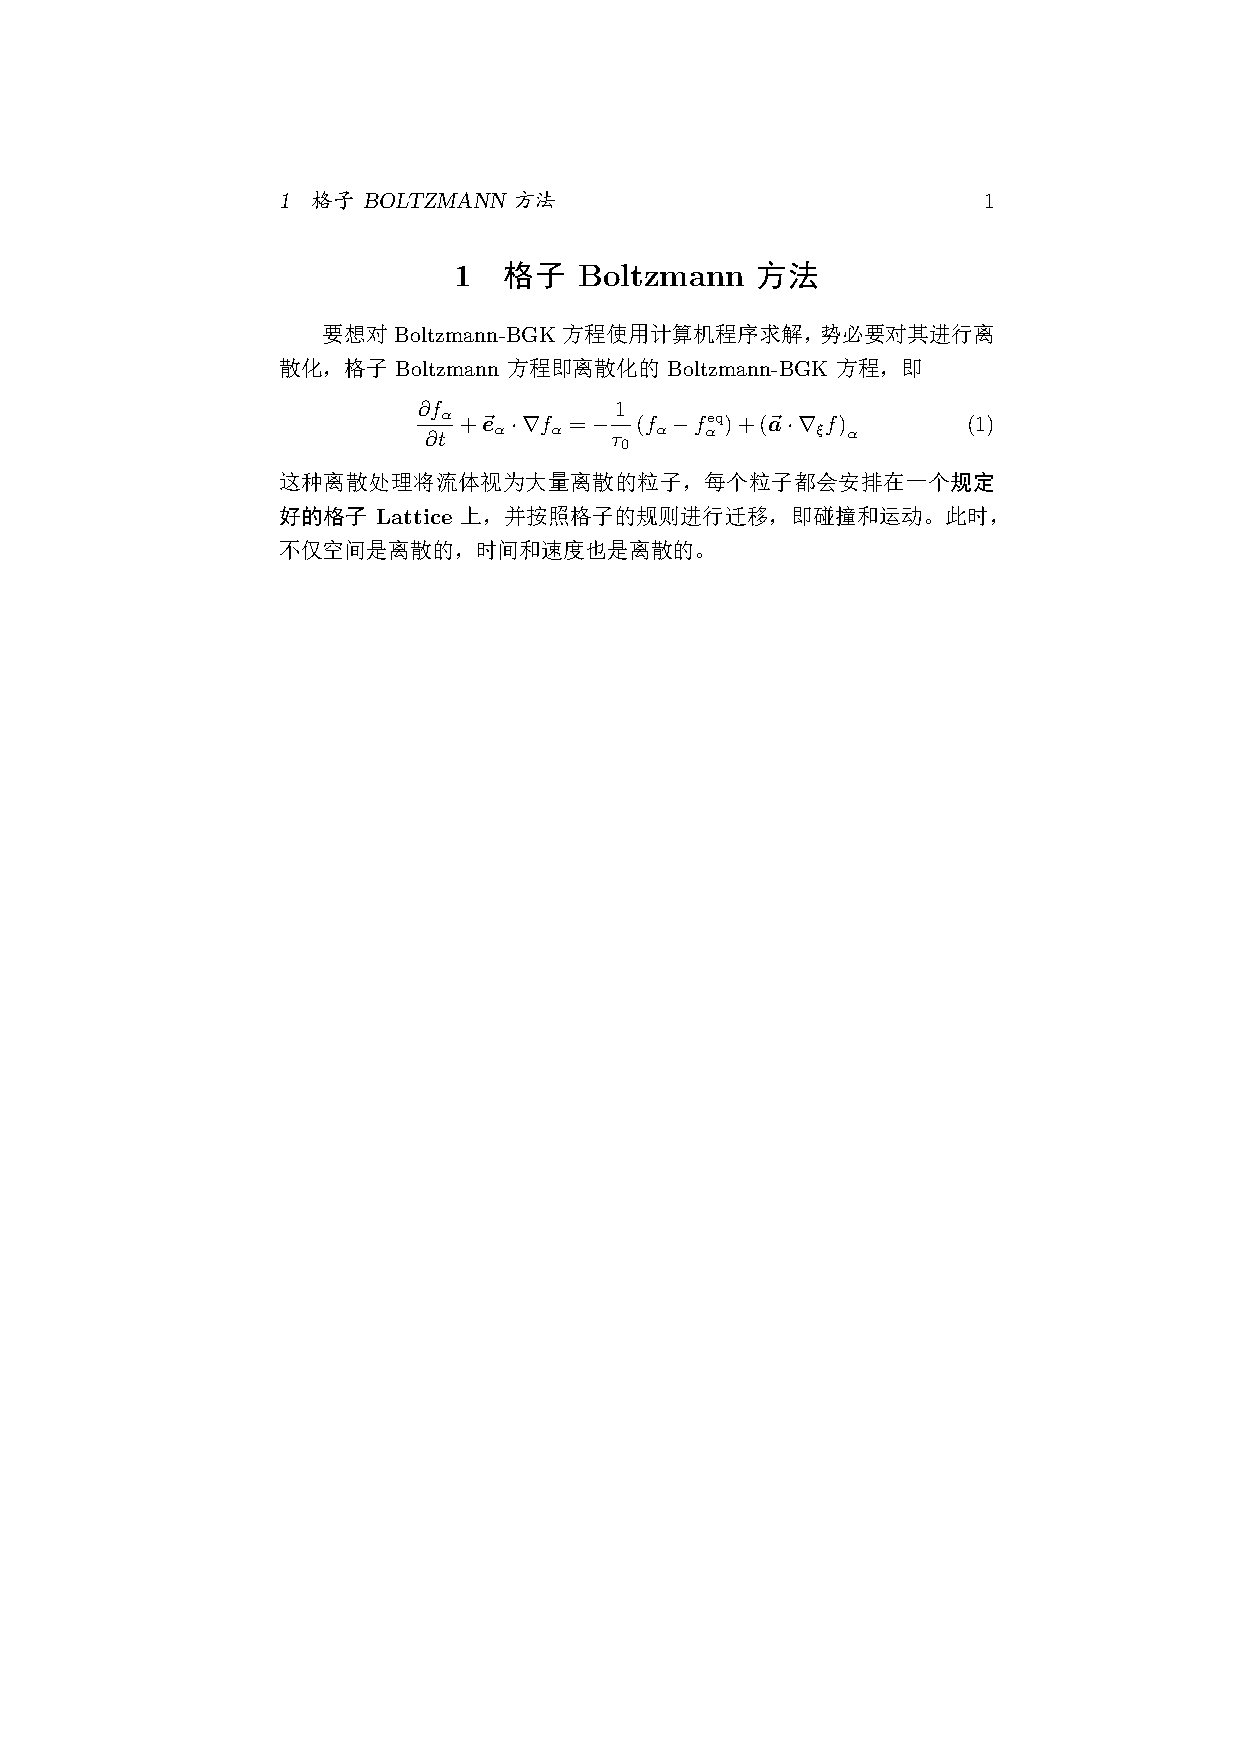
\includegraphics[scale=0.7]{figures/test2.pdf}
    \end{figure}
\end{frame}

\begin{frame}[fragile]
    \frametitle{谋篇布局}
    \begin{itemize}
        \item 文档结构
              \begin{itemize}
                  \item 标题:\verb|\title|、\verb|\author|、\verb|\date| $\to$ \verb|\maketitle|
                  \item 摘要:\verb|abstract| 环境
                  \item 目录:\verb|\tableofcontents|
                  \item 章节:\verb|\chapter|、\verb|\section|、\verb|\subsection| 等
                  \item 文献:\verb|\bibliography| 或 \verb|\printbibliography|
              \end{itemize}
        \item 文档划分
              \begin{itemize}
                  \item 分文件编译:\verb|\include|、\verb|\input|
              \end{itemize}
    \end{itemize}
\end{frame}

\begin{frame}[fragile]
    \frametitle{文本标记}
    \begin{itemize}
        \item 加粗:\verb|{\bfseries ...}| 或 \verb|\textbf{...}|
        \item 倾斜:\verb|{\itshape ...}| 或 \verb|\textit{...}|
        \item 字号:\verb|\tiny|、\verb|\small|、\verb|\large|、\verb|\Large| 等
        \item 换行:\verb|\\|
        \item 缩进:\verb|\indent|
        \item 居中:\verb|\centering| 或 \verb|center| 环境
    \end{itemize}
\end{frame}

\begin{frame}[fragile]
    \frametitle{常用环境:列表}
    \begin{columns}[c]
        \begin{column}{0.5\textwidth}
            \footnotesize
            \begin{lstlisting}
\begin{enumerate}
    \item 西安交通大学的优秀学辅
    \begin{itemize}
        \item 彭康学导团
        \item 仲英学辅
        \item 钱院学辅
        \item 治学团
    \end{itemize}
    \item 吾日三省吾身
    \begin{itemize}
        \item 群内答疑乎?
        \item 共享学习链接乎?
        \item \LaTeX{}技能精进乎?
    \end{itemize}
\end{enumerate}
            \end{lstlisting}
        \end{column}
        \begin{column}{0.5\textwidth}
            \begin{enumerate}
                \item 西安交大优秀学辅
                      \begin{itemize}
                          \item 彭康学导团
                          \item 仲英学辅
                          \item 钱院学辅
                          \item 治学团
                      \end{itemize}
                \item 吾日三省吾身
                      \begin{itemize}
                          \item 群内答疑乎?
                          \item 共享学习链接乎?
                          \item \LaTeX{}技能精进乎?
                      \end{itemize}
            \end{enumerate}
        \end{column}
    \end{columns}
\end{frame}

\begin{frame}[fragile]
    \frametitle{常用环境:图片}
    \begin{columns}
        \begin{column}{0.6\textwidth}
            \begin{lstlisting}
\begin{figure}
    \centering
    % 可指定宽度、高度等选项
    
\includegraphics[scale=0.07]{figures/PKSTU-Logo.png}
    \caption{Logo of PKSTU}
    \label{fig:PKSTU-Logo}% 方便引用
\end{figure}
            \end{lstlisting}
        \end{column}
        \begin{column}{0.4\textwidth}
            \begin{figure}
                \centering
                
\includegraphics[scale=0.07]{figures/PKSTU-Logo.png}
                \caption{Logo of PKSTU}
                \label{fig:PKSTU-Logo}
            \end{figure}
        \end{column}
    \end{columns}
\end{frame}

\begin{frame}[fragile]
    \frametitle{常用环境:表格}
    \begin{columns}
        \begin{column}{0.6\textwidth}
            \scriptsize
            \begin{lstlisting}
% 导言区
\usepackage{booktabs} % 提供\toprule等命令
% 正文
\begin{table}
    \caption{彭康学导团主要群聊人数}
    \label{tab:PKSTU-members}
    % 列格式:c 居中,l 左对齐,r 右对齐
    \begin{tabular}{cc}
    \toprule
    群聊名称 & 人数 \\
    \midrule
    彭小帮2.0 & 1417 \\
    彭小帮1.0 & 1028 \\
    学导团2022成员群 & 59 \\
    \bottomrule
    \end{tabular}
\end{table}
            \end{lstlisting}
        \end{column}
        \begin{column}{0.5\textwidth}
            \begin{table}
                \small
                \caption{彭康学导团主要群聊人数}
                \label{tab:PKSTU-members}
                \begin{tabular}{cc}
                    \toprule
                    群聊名称 & 人数 \\
                    \midrule
                    彭小帮2.0 & 1417 \\
                    彭小帮1.0 & 1028 \\
                    学导团2022成员群 & 59 \\
                    \bottomrule
                \end{tabular}
            \end{table}
        \end{column}
    \end{columns}
\end{frame}
\section{数学公式}
\begin{frame}[fragile]
    \frametitle{数学模式}
    \begin{itemize}
        \item<+-> 一切数学公式都要在数学模式下输入
            \begin{itemize}
                \item 不受外界字体命令控制
                \item 数学模式中空格不起作用
                \item 始终调用 \pkg{amsmath} 宏包
            \end{itemize}
        \item<+-> 行内公式
            \begin{itemize}
                \item 用一对美元符号:\verb|$...$|
                \item \verb|$pV=nRT$| $\to$ $pV=nRT$
            \end{itemize}
        \item<+-> 行间公式
            \begin{itemize}
                \item 无编号:\verb|\[...\]| 或 \verb|equation*| 环境
                \item 编号:\verb|equation| 环境
                \item \textcolor{tip}{不推荐用 \texttt{\$\$...\$\$}}
            \end{itemize}
        \item<+-> 偷个懒
            \begin{itemize}
                \item Mathpix 截图识别 \link{https://mathpix.com/}
                \item 不建议完全依赖,需要氪金。
            \end{itemize}
    \end{itemize}
\end{frame}

\begin{frame}[fragile]
    \frametitle{结构}
    \begin{itemize}
        \item<+-> 上、下标
            \begin{itemize}
                \item \verb|^| 和 \verb|_|:\verb|f^ab| 和 \verb|f^{ab}|,\verb|{e^x}^2| 和 \verb|e^{x^2}|
                \item 配合积分、求和、极限使用:\verb|\int|、\verb|\sum|、\verb|\lim|
            \end{itemize}
        \item<+-> 分式
            \begin{itemize}
                \item \verb|\frac{<分子>}{<分母>}|
                \item 行内分式、小分式不好看:改用 \verb|a/b|,或改用独显公式\verb|\displaystyle|
            \end{itemize}
        \item<+-> 根式
            \begin{itemize}
                \item \verb|\sqrt[<次数>]{<内容>}|
                \item 复杂情况改用分数指数:\verb|{...}^{1/n}|
            \end{itemize}
        \item<+-> 矩阵与行列式
            \begin{itemize}
                \item \verb|matrix|、\verb|pmatrix|、\verb|vmatrix| 等环境
                \item 语法类似表格:\verb|&| 分列,\verb|\\| 换行
            \end{itemize}
    \end{itemize}
\end{frame}

\begin{frame}[fragile]
    \frametitle{括号与定界符}
    \begin{itemize}
        \item<+-> 基本括号
            \begin{itemize}
                \item \verb|(...)|、\verb|[...]|、\verb|\{...\}|、
                \item 绝对值:\lstinline+|...|+
            \end{itemize}
        \item<+-> 自动调节
            \begin{itemize}
                \item \verb|\left(...\right)|、\verb|\left[...\right]|、\verb|\left{...\right}|
                \item \pkg{physics}宏包的 \verb|\qty| 命令
            \end{itemize}
        \item<+-> 手动调节
            \begin{itemize}
                \item \verb|\big|、\verb|\Big|、\verb|\bigg|、\verb|\Bigg|
            \end{itemize}
    \end{itemize}
\end{frame}

\begin{frame}[fragile]
    \frametitle{符号与字体}
    \begin{itemize}
        \item 寻找符号
              \begin{itemize}
                  \item 最常用的额外字体包:\pkg{amssymb}
                  \item \LaTeX{}编辑器和插件提供常见符号命令
              \end{itemize}
        \item 数学字体
              \begin{itemize}
                  \item 被广泛使用的「Times New Roman」:\pkg{newtxmath} 宏包
                  \item 加粗:使用 \pkg{bm} 宏包的 \verb|\bm| 命令
              \end{itemize}
        \item 新方案:\pkg{unicode-math}
    \end{itemize}
\end{frame}

\begin{frame}[fragile]
    \frametitle{多行公式}
    \begin{itemize}
        \item 以下均要求 \pkg{amsmath} 宏包
        \item 独立数学环境
              \begin{itemize}
                  \item \verb|align| 环境,\verb|&| 加在需要对齐处
              \end{itemize}
        \item 内联数学环境
              \begin{itemize}
                  \item 条件 \verb|cases|、多行对齐 \verb|split|
              \end{itemize}
    \end{itemize}
\end{frame}

\begin{frame}[fragile]
    \frametitle{V个公式,看看实力}
    \small
    \begin{equation*}
        \displaystyle \oint_{L_1}^{L_2}\mathcal{D}[x(t)]\sqrt{\frac{\displaystyle3\pi^2-\sum_{q=0}^{\infty}(z+\hat L)^{q}\exp(iq^2 \hbar x)}{\displaystyle \prod_{m=0}^{\infty}\left(\bm{\Lambda}_{j_1j_2}^{i_1i_2}\Gamma_{i_1i_2}^{j_1j_2}\hookrightarrow\vec D\cdot \mathbf{P}  \right)}}
        ={\widetilde{\left\langle \frac{\notin \emptyset}{\varpi\alpha_{k\uparrow}}\middle\vert \frac{\partial_\mu T_{\mu\nu}}{2}\right\rangle}},\forall z \in \mathbb{R}
    \end{equation*}
    \scriptsize
    \begin{lstlisting}
\begin{equation}
    \displaystyle \oint_{L_1}^{L_2}\mathcal{D}[x(t)]\sqrt{\frac{\displaystyle 3\pi^2-\sum_{q=0}^{\infty}(z+\hat L)^{q}\exp(iq^2 \hbar x)}{\displaystyle \prod_{m=0}^{\infty}\left(\bm{\Lambda}_{j_1j_2}^{i_1i_2}\Gamma_{i_1i_2}^{j_1j_2}\hookrightarrow\vec D\cdot \mathbf{P} \right)}}={\widetilde{\left\langle \frac{\notin \emptyset}{\varpi\alpha_{k\uparrow}}\middle\vert\frac{\partial_\mu T_{\mu\nu}}{2}\right\rangle}},\forall z \in \mathbb{R}
\end{equation}
    \end{lstlisting}
\end{frame}
\section{使用模板}

\begin{frame}[fragile]
    \frametitle{模板}
    \begin{itemize}
        \item<+-> 是什么?
            \begin{itemize}
                \item 设计好的格式框架
                \item 专注于内容
                \item 需要了解并遵循模板特性
            \end{itemize}
        \item<+-> 有哪些?
            \begin{itemize}
                \item 期刊:\pkg{elsarticle}、\pkg{IEEEtran}……
                \item 学位论文:\pkg{xjtuthesis} \link{https://github.com/Aetf/xjtuthesis.git}、\pkg{thuthesis} \link{https://github.com/tuna/thuthesis.git}、\pkg{ustcthesis} \link{https://github.com/ustctug/ustcthesis.git}……
            \end{itemize}
        \item<+-> 怎么用?
            \begin{itemize}
                \item \verb|\documentclass{...}|,配置参数,照常编写
                \item \textcolor{tip}{看文档!}
            \end{itemize}
        \item<+-> 去哪里找?
            \begin{itemize}
                \item CTAN \link{https://ctan.org} 或 GitHub \href{https://github.com}{\faGithub}
            \end{itemize}
    \end{itemize}
\end{frame}

\begin{frame}[standout]
    \huge 请务必先读文档! \\[1ex]
    \footnotesize \faWindows{} + {\ttfamily R} $\to$ \texttt{texdoc \textit{package}}
\end{frame}
\begin{frame}[fragile]
    \frametitle{参考文献与扩展阅读}
    \scriptsize
    \begin{multicols}{2}
        \newcommand\TAG[1]{\CASE{[#1]}}
        \begin{thebibliography}{99}
            \scriptsize
            \bibitem{}
            \scriptsize
            刘海洋.\LaTeX{} 入门 \TAG{M}, 2013. 北京:电子工业出版社
            \scriptsize
            \bibitem{}
            \scriptsize
            Oetiker T, Partl H, Hyna I and Schlegl E.\CTeX{} 开发小组~译.一份(不太)简短的 \LaTeXe{} 介绍:或 111 分钟了解 \LaTeXe{} \TAG{EB/OL}, 2021. \link{https://ctan.org/pkg/lshort-zh-cn}
            \scriptsize
            \bibitem{}
            \scriptsize
            黄新刚(包太雷).\LaTeX{} Notes: 雷太赫排版系统简介(第二版) \TAG{EB/OL}, 2021. \href{https://github.com/huangxg/lnotes}{\faGithub}
            \scriptsize
            \bibitem{}
            \scriptsize
            陈晟祺.清华大学图书馆:如何使用 \LaTeX{} 排版论文 \TAG{EB/OL}, 2021. \href{https://github.com/tuna/thulib-latex-talk}{\faGithub}
            \scriptsize
            \bibitem{}
            \scriptsize
            吴伟健,李子龙.上海交通大学图书馆:如何使用 \LaTeX{} 排版论文 \TAG{EB/OL}, 2022. \href{https://github.com/sjtug/sjtulib-latex-talk}{\faGithub}
            \scriptsize
            \bibitem{}
            \scriptsize
            刘海洋.\LaTeX{} 不快速的入门 \TAG{EB/OL}, 2020. Video: \href{https://www.bilibili.com/video/BV1s7411U7Pr}{\faVideo}
            \scriptsize
            \bibitem{}
            \scriptsize
            林莲枝.漫谈 \LaTeX{} 排版常见概念误区:别把 \LaTeX{} 当 Word 用!\TAG{EB/OL}, 2018. Video: \href{https://www.bilibili.com/video/BV1r4411o7KJ}{\faVideo}\quad
            PDF: \href{http://static.latexstudio.net/wp-content/uploads/2018/03/LianTze-presentation-0320-forReading.pdf}{\faDownload}
            \scriptsize
            \bibitem{}
            \scriptsize
            熊煜.南京大学:现代\LaTeX{} 从入门到入门 \TAG{EB/OL}, 2022. \href{https://git.nju.edu.cn/atXYblip/latex-lecture}{\faGitlab}
        \end{thebibliography}
    \end{multicols}
\end{frame}
\begin{frame}{关于}
    \vspace*{0.2cm}
    \begin{center}
        \huge
        \href{https://creativecommons.org/licenses/by-sa/4.0/}{\faCreativeCommons\,\faCreativeCommonsBy\,\faCreativeCommonsSa}
    \end{center}

    \medskip
    \footnotesize
    项目地址 \href{https://github.com/PKSTU/}{\faGithub}\\
    许可证 (LICENSE):署名-相同方式共享 4.0 国际 (CC BY-SA 4.0)

    \begin{center}
        \rule{0.8\textwidth}{1pt}
    \end{center}

    \medskip
    特别鸣谢:
    \scriptsize
    \begin{itemize}
        \item 曾祥东《现代 \LaTeX{} 入门讲座》 \href{https://github.com/stone-zeng/latex-talk}{\faGithub}
        \item 黄晨成《一份其实很短的 \LaTeX{} 入门文档》 \link{https://liam.page/2014/09/08/latex-introduction/}
        \item 熊煜《现代 \LaTeX{} 从入门到入门》 \href{https://git.nju.edu.cn/atXYblip/latex-lecture}{\faGitlab}
    \end{itemize}

    % \vspace{2cm}
    \begin{flushleft}
        \tiny
        Beamer 主题:metropolis \link{https://ctan.org/pkg/pgfornament-han} \\
        正文字体:方正清刻本悦宋简体 + Palatino \\
        等宽字体:Consolas
    \end{flushleft}
    \vspace{-0.5cm}
\end{frame}
\begin{frame}[standout]
    \huge \huge \textbf{\texttt{\textbackslash Bye[to]\{everyone\}}}
\end{frame}

\end{document}